\begin{frame}
 \begin{figure}[h]
  \centering
  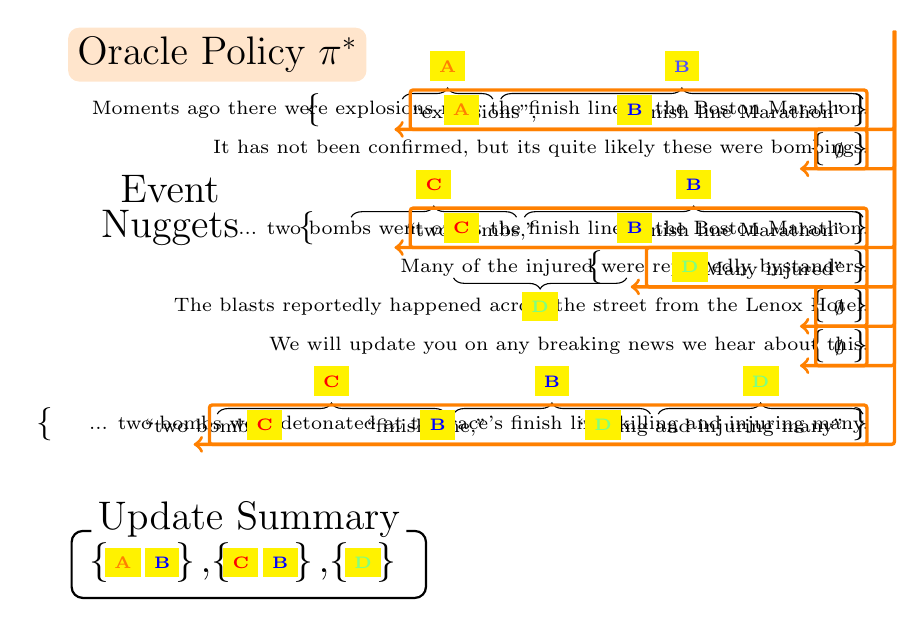
\begin{tikzpicture}
    \tikzstyle{sent}=[align=left]
    \tikzstyle{doc}=[rectangle,rounded corners,draw=black, very thick]

    \visible<-3>{
   \node at (0.5,6) [align=left] {\Large Event} ;
   \node at (0.5,5.5) [align=left] {\Large Nuggets} ;
    }
  \visible<-2>{

    \node[sent,left] at (9.5, 7) {\fontsize{7}{11}\selectfont Moments ago there were 
        explosions near the finish line of the Boston Marathon.}; 
    \node[sent,left] at (9.5, 6.5) {\fontsize{7}{11}\selectfont It has not been confirmed, 
        but its quite likely these were bombings.};
    
    \node[sent,left] at (9.5, 5.5) {\fontsize{7}{11}\selectfont ... two bombs went off at the 
        finish line of the Boston  Marathon.};
    \node[sent,left] at (9.5, 5) {\fontsize{7}{11}\selectfont Many of the injured were 
        reportedly bystanders.};
    \node[sent,left] at (9.5, 4.5) {\fontsize{7}{11}\selectfont The blasts reportedly happened 
        across the street from the Lenox Hotel.};
    \node[sent,left] at (9.5, 4) {\fontsize{7}{11}\selectfont We will update you on any 
        breaking news we hear about this.};

    \node[sent,left] at (9.5, 3) {\fontsize{7}{11}\selectfont ... two bombs were detonated at 
        the race's finish line, killing and injuring many.};
%    \node[sent,left] at (9.5, 2.5) {\fontsize{7}{11}\selectfont ... two more explosive devices
%         have been found.};
%    \node[sent,left] at (9.5, 2.0) {\fontsize{7}{11}\selectfont The White House says President 
%        Obama has been notified about the explosions.};
%
%    \node[sent,left] at (9.5, 1.0) {\fontsize{7}{11}\selectfont NBC news reports that 
%        ``multiple explosive devices'' have been found in Boston.};
%    \node[sent,left] at (9.5, 0.5) {\fontsize{7}{11}\selectfont Boston police report
%        that two people were killed and at least 22 injured.};
%    \node[sent,left] at (9.5, 0.0) {\fontsize{7}{11}\selectfont More on this
%        story as it develops.};
    }
%    \node[text=green] at (10.3, 7.05) {\Huge $\boldsymbol{+}$ };
%    \node[text=red] at (10.3, 6.50) {\Huge $\boldsymbol{-}$ };
        \visible<2>{
    \draw [decorate,decoration={brace,amplitude=4pt,raise=1pt},yshift=0pt]
    (3.45,7.1) -- (4.6,7.1) 
    node[rectangle,fill=yellow,midway,xshift=0.0cm,yshift=0.45cm,text=orange] 
    {\fontsize{6}{8}\selectfont \textbf{A}};
    \draw [decorate,decoration={brace,amplitude=4pt,raise=1pt},yshift=0pt]
    (4.7,7.1) -- (9.3,7.1) 
    node[rectangle,fill=yellow,midway,xshift=0.0cm,yshift=0.45cm,text=blue!70] 
    {\fontsize{6}{8}\selectfont \textbf{B}};
    \draw [decorate,decoration={brace,amplitude=4pt,raise=1pt},yshift=0pt]
    (2.8,5.6) -- (4.9,5.6) 
    node[rectangle,fill=yellow,midway,xshift=0.0cm,yshift=0.45cm,text=red] 
    {\fontsize{6}{8}\selectfont \textbf{C}};
    \draw [decorate,decoration={brace,amplitude=4pt,raise=1pt},yshift=0pt]
    (5,5.6) -- (9.3,5.6) 
    node[rectangle,fill=yellow,midway,xshift=0.0cm,yshift=0.45cm,text=blue] 
    {\fontsize{6}{8}\selectfont \textbf{B}};


    \draw [decorate,decoration={brace,amplitude=4pt,raise=1pt,mirror},yshift=0pt]
    (4.1,4.9) -- (6.3,4.9) 
    node[rectangle,fill=yellow,midway,xshift=0.0cm,yshift=-0.4cm,text=green!50] 
    {\fontsize{6}{8}\selectfont \textbf{D}};

  
    \draw [decorate,decoration={brace,amplitude=4pt,raise=1pt,},yshift=0pt]
    (1.1,3.1) -- (4.0,3.1) 
    node[rectangle,fill=yellow,midway,xshift=0.0cm,yshift=0.45cm,text=red] 
    {\fontsize{6}{8}\selectfont \textbf{C}};
    \draw [decorate,decoration={brace,amplitude=4pt,raise=1pt,},yshift=0pt]
    (4.1,3.1) -- (6.6,3.1) 
    node[rectangle,fill=yellow,midway,xshift=0.0cm,yshift=0.45cm,text=blue] 
    {\fontsize{6}{8}\selectfont \textbf{B}};
    \draw [decorate,decoration={brace,amplitude=4pt,raise=1pt,},yshift=0pt]
    (6.7,3.1) -- (9.3,3.1) 
    node[rectangle,fill=yellow,midway,xshift=0.0cm,yshift=0.45cm,text=green!50] 
    {\fontsize{6}{8}\selectfont \textbf{D}};


%    \draw [decorate,
%           decoration={brace,mirror,amplitude=4pt,raise=1pt,aspect=.70}]
%    (4.4,2.45) -- (9.3,2.45) 
%    node[rectangle,fill=yellow,midway,xshift=1.0cm,yshift=-0.4cm,text=purple] 
%    {\fontsize{6}{8}\selectfont \textbf{E}};
%
%
%    \draw [decorate,
%           decoration={brace,mirror,amplitude=4pt,raise=1pt,},yshift=0pt]
%    (3.1,1.90) -- (9.3,1.90) 
%    node[rectangle,fill=yellow,midway,xshift=0.0cm,yshift=-0.4cm,text=magenta] 
%    {\fontsize{6}{8}\selectfont \textbf{F}};
%
%    \draw [decorate,
%           decoration={brace,mirror,amplitude=4pt,raise=1pt,aspect=.2}]
%    (4.4,.40) -- (9.3,0.40) 
%    node[rectangle,fill=yellow,midway,xshift=-42pt,yshift=-0.4cm,text=green!50] 
%    {\fontsize{6}{8}\selectfont \textbf{D}};
%
%    \draw [decorate,
%           decoration={brace,amplitude=4pt,raise=1pt,aspect=.2},xshift=0pt,]
%    (3.4,1.1) -- (9.3,1.1) 
%    node[rectangle,fill=yellow,midway,xshift=-51pt,yshift=0.45cm,text=purple] 
%    {\fontsize{6}{8}\selectfont \textbf{E}};

    }


  \visible<3->{

    \node[sent,left] at (9.5, 7) {\fontsize{7}{11}\selectfont 
    {\large\{} ~~~~~~~~~~ ``explosions'', ~~~~~~~~~~ ``finish line Marathon'' 
        {\large\}}}; 

    \node[sent,left] at (9.5, 6.5) 
    {\fontsize{7}{11}\selectfont {\large\{} $\emptyset$ {\large\}}};
    
    \node[sent,left] at (9.5, 5.5) 
    {\fontsize{7}{11}\selectfont 
    {\large\{} ~~~~~~~~~~ ``two bombs,'' ~~~~~~~~~~ ``finish line Marathon'' 
        {\large\}}};

    \node[sent,left] at (9.5, 5) 
    {\fontsize{7}{11}\selectfont {\large\{} ~~~~~~~~~~ ``Many injured''
        {\large\}}};

    \node[sent,left] at (9.5, 4.5) {\fontsize{7}{11}\selectfont 
    {\large\{} $\emptyset$ {\large\}}};
    \node[sent,left] at (9.5, 4) {\fontsize{7}{11}\selectfont 
    {\large\{} $\emptyset$ {\large\}}};

    \node[sent,left] at (9.5, 3) {\fontsize{7}{11}\selectfont 
        {\large\{}   
          ~~~~~~~~~~ ``two bombs,'' ~~~~~~~~~~ ``finish line,'' 
          ~~~~~~~~~~ ``killing and injuring many'' 
    {\large\}}};

%    \node[sent,left] at (9.5, 2.5) {\fontsize{7}{11}\selectfont 
%    {\large\{} ~~~~~~~~~~ ``two more found'' {\large\}}};
%    \node[sent,left] at (9.5, 2.0) {\fontsize{7}{11}\selectfont 
%    {\large\{} ~~~~~~~~~~ ``Obama has been notified'' {\large\}}};
%
%    \node[sent,left] at (9.5, 1.0) {\fontsize{7}{11}\selectfont 
%    {\large\{} ~~~~~~~~~~ ``multiple explosive devices found'' {\large\}}};
%    \node[sent,left] at (9.5, 0.5) {\fontsize{7}{11}\selectfont 
%        {\large\{} ~~~~~~~~~~ ``people killed and injured'' {\large\}}};
%    \node[sent,left] at (9.5, 0.0) {\fontsize{7}{11}\selectfont 
%    {\large\{} $\emptyset$ {\large\}}};


    \node at (4.2,7.0) [rectangle,fill=yellow,text=orange] 
    {\fontsize{6}{8}\selectfont \textbf{A}};

    \node at (6.4,7.0) [rectangle,fill=yellow,text=blue] 
    {\fontsize{6}{8}\selectfont \textbf{B}};

    \node at (4.2,5.5) [rectangle,fill=yellow,text=red] 
    {\fontsize{6}{8}\selectfont \textbf{C}};
    
    \node at (6.4,5.5) [rectangle,fill=yellow,text=blue] 
    {\fontsize{6}{8}\selectfont \textbf{B}};

    \node at (7.1,5.0) [rectangle,fill=yellow,text=green!50] 
    {\fontsize{6}{8}\selectfont \textbf{D}};

    \node at (1.7,3.0) [rectangle,fill=yellow,text=red] 
    {\fontsize{6}{8}\selectfont \textbf{C}};

    \node at (3.9,3.0) [rectangle,fill=yellow,text=blue] 
    {\fontsize{6}{8}\selectfont \textbf{B}};

    \node at (6,3.0) [rectangle,fill=yellow,text=green!50] 
    {\fontsize{6}{8}\selectfont \textbf{D}};
%
%    \node at (6.9,2.5) [rectangle,fill=yellow,text=purple] 
%    {\fontsize{6}{8}\selectfont \textbf{E}};
%
%    \node at (5.8,2) [rectangle,fill=yellow,text=magenta] 
%    {\fontsize{6}{8}\selectfont \textbf{F}};
%
%    \node at (5.1,1) [rectangle,fill=yellow,text=purple] 
%    {\fontsize{6}{8}\selectfont \textbf{E}};
%    
%    \node at (5.8,.5) [rectangle,fill=yellow,text=green!50] 
%    {\fontsize{6}{8}\selectfont \textbf{D}};
}

 \visible<5-6>{
    \draw[orange,very thick,rounded corners=1pt,->] 
        (9.7,8) -- (9.7,6.75) -- (3.35,6.75);
    \draw[orange,very thick,rounded corners=1pt] 
        (3.55,7.25) rectangle (9.35, 6.75);
  }
  \visible<6->{ 
      \node at (3.15, 7) [text=green] 
      {$\Plus$ }; 
    \node at (-.4,1.25) [text=black]
    {\fontsize{6}{8}\selectfont {\Large\{} };
    \node at (-.1,1.25) [rectangle,fill=yellow,text=orange] 
    {\fontsize{6}{8}\selectfont \textbf{A}};
    \node at (.4,1.25) [rectangle,fill=yellow,text=blue] 
    {\fontsize{6}{8}\selectfont \textbf{B}};
    \node at (.7,1.25) [text=black]
    {\fontsize{6}{8}\selectfont {\Large\}} };
  }



 \visible<7-8>{
    \draw[orange,very thick,rounded corners=1pt,->] 
        (9.7,8) -- (9.7,6.25) -- (8.5,6.25);
    \draw[orange,very thick,rounded corners=1pt] 
        (8.7,6.75) rectangle (9.35, 6.25);
  }
  \visible<8->{ 
      \node at (8.3, 6.4) [text=red] 
      {$\Minus$ }; 
  }

 \visible<9-10>{
    \draw[orange,very thick,rounded corners=1pt,->] 
        (9.7,8) -- (9.7,5.25) -- (3.35,5.25);
    \draw[orange,very thick,rounded corners=1pt] 
        (3.55,5.75) rectangle (9.35, 5.25);
  }
  \visible<10->{ 
      \node at (3.15, 5.5) [text=green] 
      {$\Plus$ }; 

    \node at (1.,1.25) [text=black]
    {\fontsize{6}{8}\selectfont {\Large ~,\{} };
    \node at (1.4,1.25) [rectangle,fill=yellow,text=red] 
    {\fontsize{6}{8}\selectfont \textbf{C}};
    \node at (1.9,1.25) [rectangle,fill=yellow,text=blue] 
    {\fontsize{6}{8}\selectfont \textbf{B}};
    \node at (2.2,1.25) [text=black]
    {\fontsize{6}{8}\selectfont {\Large\}} };
  }

 \visible<11-12>{
    \draw[orange,very thick,rounded corners=1pt,->] 
        (9.7,8) -- (9.7,4.75) -- (6.35,4.75);
    \draw[orange,very thick,rounded corners=1pt] 
        (6.55,5.25) rectangle (9.35, 4.75);
  }
  \visible<12->{ 
      \node at (6.15, 5) [text=green] 
      {$\Plus$ }; 
    \node at (2.5,1.25) [text=black]
    {\fontsize{6}{8}\selectfont {\Large ~,\{} };
    \node at (2.95,1.25) [rectangle,fill=yellow,text=green!50] 
    {\fontsize{6}{8}\selectfont \textbf{D}};
    \node at (3.25,1.25) [text=black]
    {\fontsize{6}{8}\selectfont {\Large\}} };
  }

 \visible<13-14>{
    \draw[orange,very thick,rounded corners=1pt,->] 
        (9.7,8) -- (9.7,4.25) -- (8.5,4.25);
    \draw[orange,very thick,rounded corners=1pt] 
        (8.7,4.75) rectangle (9.35, 4.25);
  }
  \visible<14->{ 
      \node at (8.3, 4.45) [text=red] 
      {$\Minus$ }; 
  }

 \visible<15-16>{
    \draw[orange,very thick,rounded corners=1pt,->] 
        (9.7,8) -- (9.7,3.75) -- (8.5,3.75);
    \draw[orange,very thick,rounded corners=1pt] 
        (8.7,4.25) rectangle (9.35, 3.75);
  }
  \visible<16->{ 
      \node at (8.3, 3.95) [text=red] 
      {$\Minus$ }; 
  }



 \visible<17-18>{
    \draw[orange,very thick,rounded corners=1pt,->] 
        (9.7,8) -- (9.7,2.75) -- (.8,2.75);
    \draw[orange,very thick,rounded corners=1pt] 
        (1.0,3.25) rectangle (9.35, 2.75);
  }
  \visible<18->{ 
      \node at (.6, 2.95) [text=red] 
      {$\Minus$ }; 
  }
%
% \visible<19-20>{
%    \draw[orange,very thick,rounded corners=1pt,->] 
%        (9.7,8) -- (9.7,2.25) -- (6.0,2.25);
%    \draw[orange,very thick,rounded corners=1pt] 
%        (6.2,2.75) rectangle (9.35, 2.25);
%  }
%  \visible<20->{ 
%      \node at (5.8, 2.50) [text=green] 
%      {$\Plus$ }; 
%    \node at (3.6,-.25) [text=black]
%    {\fontsize{6}{8}\selectfont {\Large ~,\{} };
%    \node at (4,-.25) [rectangle,fill=yellow,text=purple] 
%    {\fontsize{6}{8}\selectfont \textbf{E}};
%    \node at (4.3,-.25) [text=black]
%    {\fontsize{6}{8}\selectfont {\Large \}} };
%  }
%
% \visible<21-22>{
%    \draw[orange,very thick,rounded corners=1pt,->] 
%        (9.7,8) -- (9.7,1.75) -- (4.9,1.75);
%    \draw[orange,very thick,rounded corners=1pt] 
%        (5.1,2.25) rectangle (9.35, 1.75);
%  }
%  \visible<22->{ 
%      \node at (4.7, 2.0) [text=green] 
%      {$\Plus$ }; 
%    \node at (4.6,-.25) [text=black]
%    {\fontsize{6}{8}\selectfont {\Large ~,\{} };
%    \node at (5,-.25) [rectangle,fill=yellow,text=magenta] 
%    {\fontsize{6}{8}\selectfont \textbf{F}};
%    \node at (5.3,-.25) [text=black]
%    {\fontsize{6}{8}\selectfont {\Large \}} };
%  }
%
%
% \visible<23-24>{
%    \draw[orange,very thick,rounded corners=1pt,->] 
%        (9.7,8) -- (9.7,.75) -- (4.2,.75);
%    \draw[orange,very thick,rounded corners=1pt] 
%        (4.4,1.25) rectangle (9.35, .75);
%  }
%  \visible<24->{ 
%      \node at (4.0, .9) [text=red] 
%      {$\Minus$ }; 
%  }
%
% \visible<25-26>{
%    \draw[orange,very thick,rounded corners=1pt,->] 
%        (9.7,8) -- (9.7,.25) -- (5.1,.25);
%    \draw[orange,very thick,rounded corners=1pt] 
%        (5.3,0.75) rectangle (9.35, .25);
%  }
%  \visible<26->{ 
%      \node at (4.9, .4) [text=red] 
%      {$\Minus$ }; 
%  }
%
% \visible<27-28>{
%    \draw[orange,very thick,rounded corners=1pt,->] 
%        (9.7,8) -- (9.7,-.25) -- (8.5,-.25);
%    \draw[orange,very thick,rounded corners=1pt] 
%        (8.7,.25) rectangle (9.35, -.25);
%  }
%
%  \visible<28->{ 
%      \node at (8.3, -0.10) [text=red] 
%      {$\Minus$ }; 
%  }

\visible<4->{
  \node at (1.1,7.7) [fill=orange!20,rounded corners] {\Large Oracle Policy $\pi^*$ };
}
    \visible<5->{
  

  \node at (1.5,1.8) [] {\Large Update Summary};
 \draw[thick,black,rounded corners] (-.5, 1.65 ) -- (-.75, 1.65) -- (-.75,.8) 
        -- (3.75,.8) -- (3.75,1.65) -- (3.5,1.65); 
}
    \end{tikzpicture}
 \end{figure}
\end{frame}
